\begin{figure*}[t]
\begin{center}
\begin{tabular}{ >{\centering\arraybackslash} m{0.74in} || >{\centering\arraybackslash} m{5.2in} }

{\footnotesize \texttt{fireplace\_1}\break(original)} &
\showtexture{fireplace_1/frame_} \\
\hline
{\footnotesize \texttt{fireplace\_1}\break(synthesized)} &
\showtexture{fireplace_1_output/frame_} \\

\hline \hline
{\footnotesize \texttt{lava}\break(original)} &
\showtexture{lava/frame_} \\
\hline
{\footnotesize \texttt{lava}\break(synthesized)} &
\showtexture{lava_output/frame_} \\

\hline \hline
{\footnotesize \texttt{smoke\_1}\break(original)} &
\showtexture{smoke_1/frame_} \\
\hline
{\footnotesize \texttt{smoke\_1}\break(synthesized)} &
\showtexture{smoke_1_output/frame_} \\

\hline \hline
{\footnotesize \texttt{underwater}\break\texttt{vegetation\_1}\break(original)} &
\showtexture{underwater_vegetation/frame_} \\
\hline
{\footnotesize \texttt{underwater}\break\texttt{vegetation\_1}\break (synthesized)} &
\showtexture{underwater_vegetation_output/frame_} \\

\hline \hline
{\footnotesize \texttt{water\_3}\break(original)} & 
\showtexture{water_3/frame_} \\
\hline
{\footnotesize \texttt{water\_3}\break(synthesized)} & 
\showtexture{water_3_output/frame_} \\
\end{tabular}
\end{center}
\vspace{-0.45cm}
\caption[Dynamic texture synthesis success examples.]{Dynamic texture synthesis success examples. Names correspond
to files in the supplemental material.}
 \label{fig:successes}
\end{figure*}


\chapter{Evaluation \todomatthew{haven't touched yet}}\label{empirical_evaluation}

The goal of (dynamic) texture synthesis is to generate 
samples that are indistinguishable from the real input target
texture by a human observer.
In this section, we present a variety of synthesis results
including a user study to quantitatively evaluate the realism
of our results.
Given their temporal nature, our results are best viewed as 
videos.
Our two-stream architecture was implemented using TensorFlow
\cite{tabadi2015tensorflowlong}.
Results were generated using an NVIDIA Titan X (Pascal) GPU
and synthesis times ranged between one to three hours 
to generate $12$ frames with an image resolution of 
$256 \times 256$.
For our full synthesis results and source code, please refer to the
supplemental material on the project website: \url{ryersonvisionlab.github.io/two-stream-projpage}.

\section{Dynamic texture synthesis}\label{eval_dynamictexturesynthesis}

We applied our dynamic texture synthesis process 
to a wide range of textures which were selected from the 
DynTex \cite{peteri2010} database and others we collected in
the wild.
Included in our supplemental material are synthesized results
of nearly 60 different textures that encapsulate a range of
phenomena, such as flowing water, waves, clouds, fire, rippling
flags, waving plants, and schools of fish.
Some sample frames are shown in Fig.\ \ref{fig:successes}
but we encourage readers to view the videos to fully appreciate
the results.
In addition, we performed a comparison with \cite{funke2017} and 
\cite{xie2017synthesizing}.
Generally, we found our results to be qualitatively comparable or better than
these methods.
See the supplemental for more details on the comparisons with these methods.

We also generated dynamic textures incrementally, as described in
Sec.\ \ref{sec:texgen}.
The resulting textures were perceptually indistinguishable from those
generated with the batch process.
Another extension that we explored were textures with no 
discernible temporal seam between the last and first frames.
Played as a loop, these textures appear to be temporally endless.
This was achieved by assuming that the first frame follows the
final frame and adding an additional loss for the dynamics 
stream evaluated on that pair of frames.

Example failure modes of our method are presented in Fig.\ 
\ref{fig:failures}.
In general, we find that most failures result from inputs that
violate the underlying assumption of a dynamic texture, \ie, 
the appearance and/or dynamics are not spatiotemporally homogeneous.
In the case of the \texttt{escalator} example, the long edge 
structures in the appearance are not spatially homogeneous, 
and the dynamics vary due to perspective effects that
change the motion from downward to outward.
The resulting synthesized texture captures an overall downward 
motion but lacks the perspective effects and is unable to 
consistently reproduce the long edge structures.
This is consistent with previous observations
on static texture synthesis \cite{gatys2015} and suggests it is a 
limitation of the appearance stream.

Another example is the \texttt{flag} sequence where the rippling 
dynamics are relatively homogeneous across the pattern but the 
appearance  varies spatially.
As expected, the generated texture does not faithfully
reproduce the appearance; however, it does exhibit plausible 
rippling dynamics.
In the supplemental material, we include an additional failure 
case, \texttt{cranberries}, which consists of a swirling pattern.
Our model faithfully reproduces the appearance
but is unable to capture the spatially varying dynamics.
Interestingly, it still produces a result
which is statistically indistinguishable from real in our user 
study discussed below.

\paragraph*{Appearance vs.\ dynamics streams}

\begin{figure}[t]
\begin{center}
\begin{tabular}{ >{\centering\arraybackslash} m{0.55in} || >{\centering\arraybackslash} m{3.50in} }
{\footnotesize target (\texttt{fish})} & 
\showtextureshort{fish/frame_} \\
\hline \hline
{\footnotesize appearance only} &
\showtextureshort{fish_spatialonly/frame_} \\
\hline
{\footnotesize both streams} & 
\showtextureshort{fish_output/frame_} \\
\end{tabular}
\end{center}
\vspace{-0.45cm}
\caption[Dynamic texture synthesis versus texture synthesis.]{Dynamic texture synthesis versus texture synthesis.
(top row) Target texture.
(middle)
Texture synthesis without dynamics constraints shows
consistent per-frame appearance but no temporal coherence.
(bottom)
Including both streams induces consistent appearance and dynamics.
}
\label{fig:baselines}
\end{figure}



We sought to verify that the appearance and dynamics
streams were capturing complementary information.
To validate that the texture generation of multiple frames
would not induce dynamics consistent with the input, we generated
frames starting from randomly generated noise but only using the
appearance statistics and corresponding loss, \ie,
Eq.\ \ref{eq:apploss}.
As expected, this produced frames that were valid textures but
with no coherent dynamics present.
Results for a sequence containing a school of fish are shown in
Fig.\ \ref{fig:baselines}; to examine the dynamics, see 
\texttt{fish} in the supplemental material.

Similarly, to validate that the dynamics stream did not 
inadvertently include appearance information, we generated videos
using the dynamics loss only, \ie, Eq.\ \ref{eq:dynloss}.
The resulting frames had no visible appearance and had
an extremely low dynamic range, \ie, the standard
deviation of pixel intensities was 10 for values in $[0,255]$.
This indicates a general invariance to appearance and 
suggests that our two-stream dynamic texture representation
has factored appearance and dynamics, as desired.

\begin{figure}[t]
\begin{center}
\begin{tabular}{ >{\centering\arraybackslash} m{0.16\textwidth} || >{\centering\arraybackslash} m{0.80\textwidth} }
{\footnotesize \path{escalator}\break(original)} & 
\showtexture{escalator/frame_} \\
\hline
{\footnotesize \path{escalator}\break(synthesized)} & 
\showtexture{escalator_output/frame_} \\
\hline \hline
{\footnotesize \path{flag}\break(original)} &
\showtexture{flag/frame_} \\
\hline
{\footnotesize \path{flag}\break(synthesized)} &
\showtexture{flag_output/frame_} \\
\hline \hline
{\footnotesize \path{cranberries}\break(original)} &
\showtexture{cranberries/frame_} \\
\hline
{\footnotesize \path{cranberries}\break(synthesized)} &
\showtexture{cranberries_output/frame_} \\
\end{tabular}
\end{center}
\vspace{-0.45cm}
\caption[Dynamic texture synthesis failure examples.]{Dynamic texture synthesis failure examples. In
these cases, the failures are attributed to either the
appearance or the dynamics not being homogeneous.}
\label{fig:failures}
\end{figure}

\section{User study}
Quantitative evaluation for texture synthesis is a particularly
challenging task as there is no single correct output when 
synthesizing new samples of a texture.
Like in other image generation tasks (\eg, rendering), 
human perception is ultimately the most important measure.
Thus, we performed a user study to evaluate the perceived 
realism of our synthesized textures.

Similar to previous image synthesis work (\eg, \cite{chen2017}), 
we conducted a perceptual experiment with human observers to 
quantitatively evaluate our synthesis results.
We employed a forced-choice evaluation on Amazon Mechanical
Turk (AMT) with 200 different users. Each user performed 59
pairwise comparisons between a synthesized dynamic texture and 
its target.
Users were asked to choose which appeared more realistic
after viewing the textures for an exposure time sampled
randomly from discrete intervals between 0.3 and 4.8 seconds.
Measures were taken to control the experimental conditions and
minimize the possibility of low quality data.
See the supplemental material for further experimental details
of our user study.

For comparison, we constructed a baseline by using the 
flow decode layer in the dynamics loss of Eq.\ \ref{eq:dynloss}.
This corresponds with attempting to mimic the optical flow 
statistics of the texture directly.
Textures were synthesized with this model and the user study
was repeated with an additional 200 users.
To differentiate between the models, we label ``Flow decode layer'' 
and ``Concat layer'' in the figures to describe our baseline and 
final model, respectively.

The results of this study are summarized in
Fig.\ \ref{fig:pairwise_alltextures} which shows user accuracy in
differentiating real versus generated textures as a function of
time for both methods.
Overall, users are able to correctly identify the real texture
$66.1\% \pm 2.5\%$ of the time for brief 
exposures of 0.3 seconds.
This rises to $79.6\% \pm 1.1\%$ with exposures of 1.2 seconds 
and higher.
Note that ``perfect'' synthesis results would have an accuracy
of $50\%$, indicating that users were unable to differentiate 
between the real and generated textures and higher accuracy 
indicating less convincing textures.

The results clearly show that the use of the concatenation 
layer activations is far more effective than the flow decode 
layer.
This is not surprising as optical flow alone is known to be 
unreliable on many textures, particularly those with
transparency or chaotic motion (\eg, water, smoke, flames, etc.).
Also evident in these results is the time-dependant nature of 
perception for textures from both models.
Users' ability to identify the generated texture improved as 
exposure times increased to 1.2 seconds and remained relatively 
flat for longer exposures.

To better understand the performance of our approach,
we grouped and analyzed the results in terms of
appearance and dynamics characteristics.
For appearance we used the taxonomy
presented in \cite{lin2006quantitative} and grouped textures as
either regular/near-regular (\eg, periodic tiling and brick wall), 
irregular (\eg, a field of flowers), or
stochastic/near-stochastic (\eg, tv static or water).
For dynamics we grouped textures as either 
spatially-consistent (\eg, closeup of rippling sea water) or 
spatially-inconsistent (\eg, rippling sea water juxtaposed 
with translating clouds in the sky).
Results based on these groupings can be seen in
Fig.\ \ref{fig:pairwise_grouped}.

\begin{figure}[t]
	\centering
    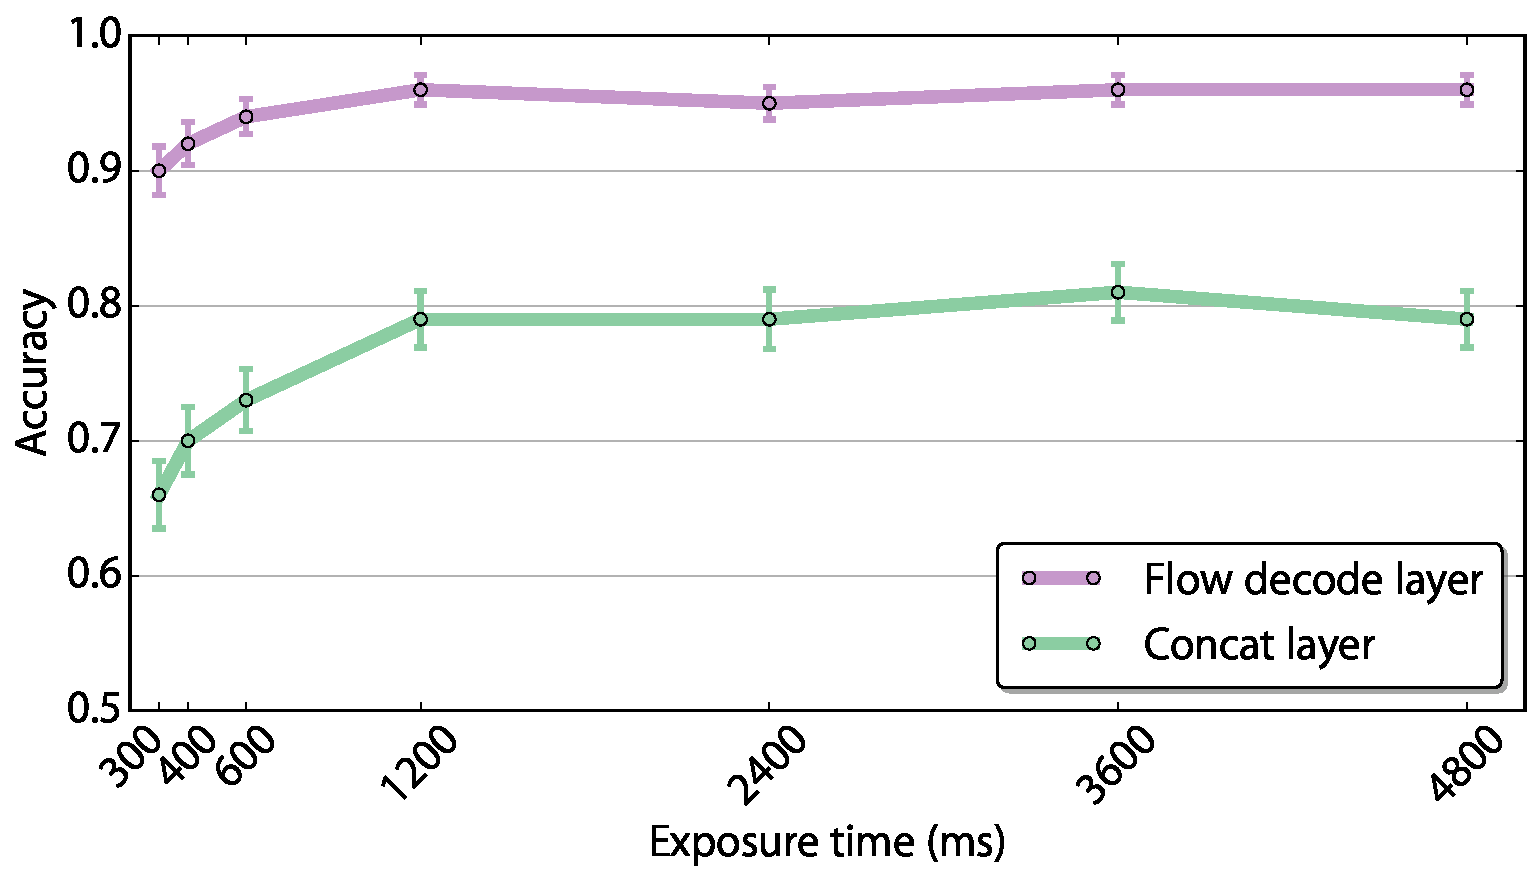
\epsfig{file=alltextures_approvedworkers.pdf, width = 0.9\textwidth}
	\caption[Time-limited pairwise comparisons across all textures]{Time-limited pairwise comparisons across all textures with $95\%$ statistical confidence intervals.}
	\label{fig:pairwise_alltextures}
\end{figure}



A full breakdown of the user study results by texture and 
grouping can be found in the supplemental material.
Here we discuss some of the overall trends.
Based on appearance it is clear that textures with
large-scale  spatial consistencies (regular, near-regular, 
and irregular textures) tend to perform poorly.
Examples being \texttt{flag} and \texttt{fountain\_2} with
user accuracies of $98.9\% \pm 1.6\%$ and $90.8\% \pm 4.3\%$ 
averaged across all exposures, respectively.
This is not unexpected and is a fundamental limitation of the 
local nature of the Gram matrix representation used in the 
appearance stream which was observed in static texture synthesis 
\cite{gatys2015}.
In contrast, stochastic and near-stochastic textures 
performed significantly better as their smaller-scale local 
variations are well captured by the appearance stream, for 
instance \texttt{water\_1} and \texttt{lava} which had 
average accuracies of $53.8\% \pm 7.4\%$ and
$55.6\% \pm 7.4\%$, respectively, making them both 
statistically indistinguishable from real.

\begin{figure}[t]
	\centering
	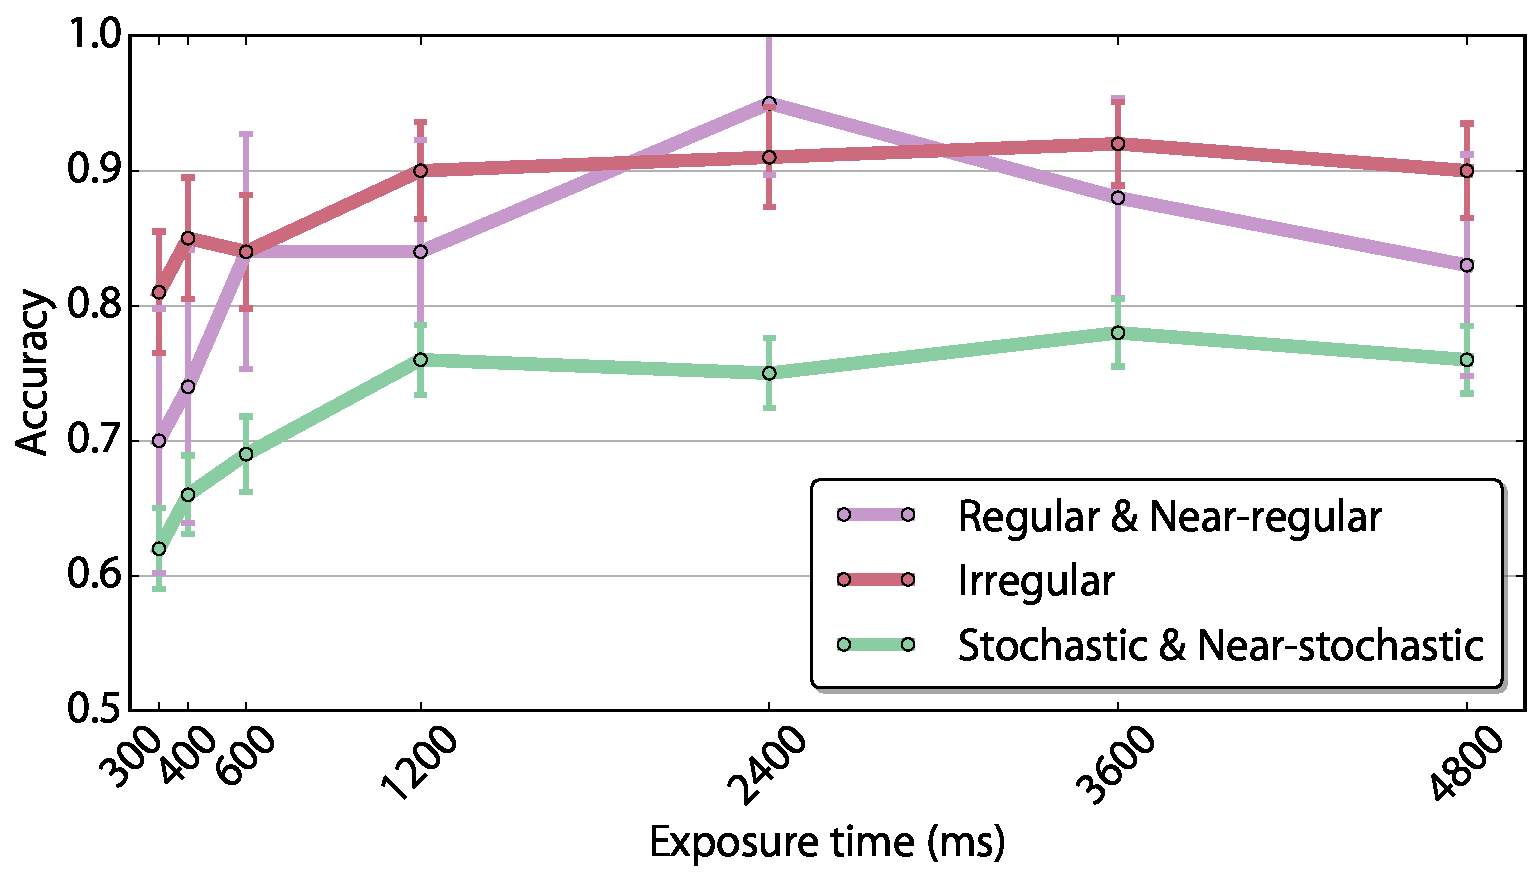
\epsfig{file=concat_appearance.pdf, width = 0.9\textwidth}\\
    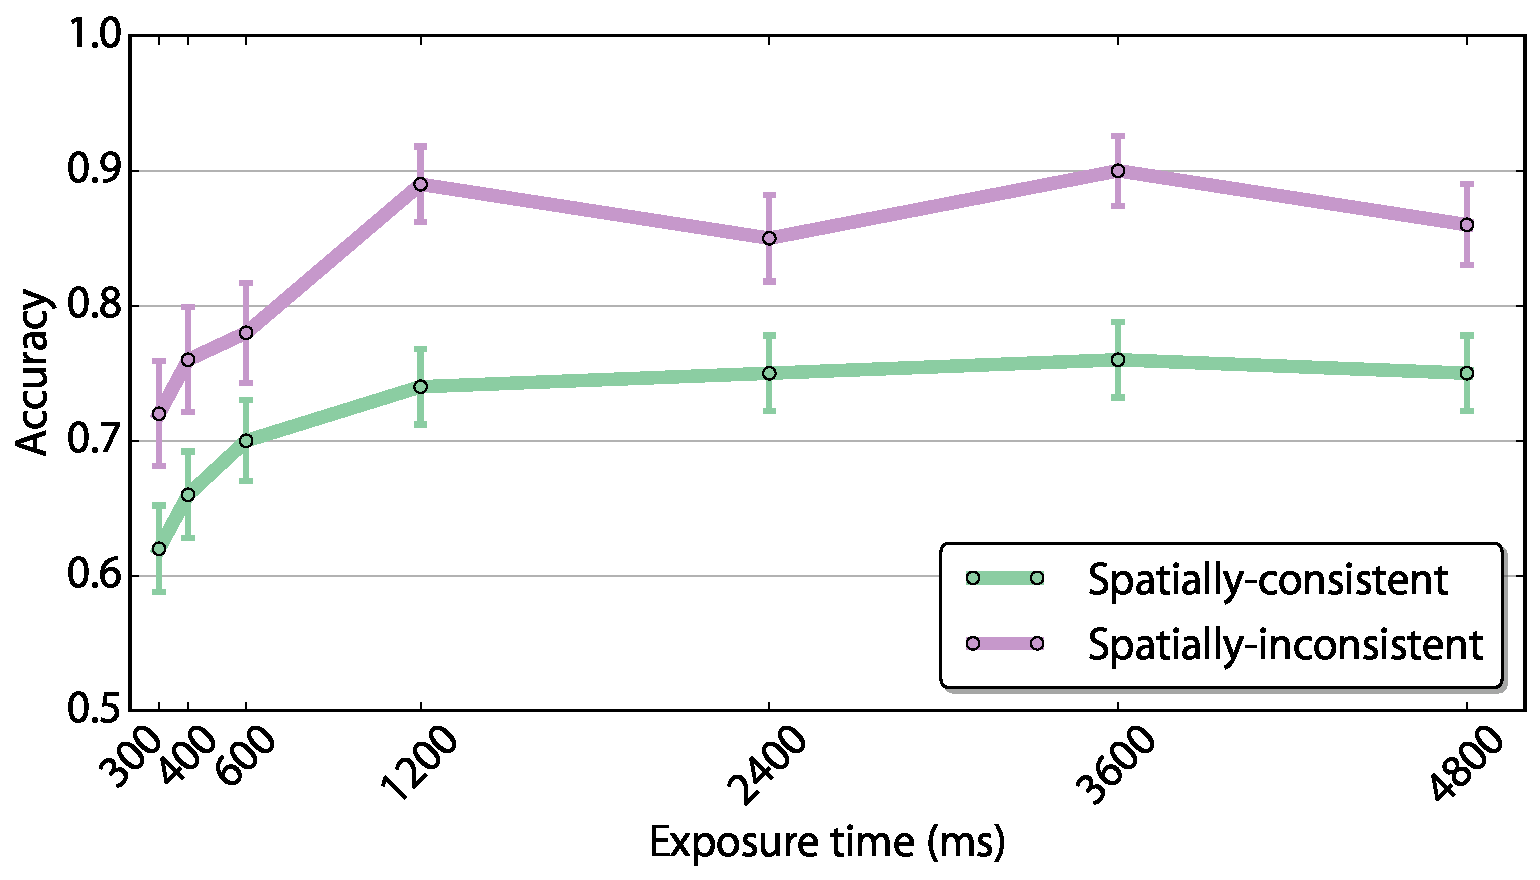
\epsfig{file=concat_dynamics.pdf, width = 0.9\textwidth}
	\caption[Time-limited pairwise comparisons across all textures, grouped by appearance and dynamics.]{Time-limited pairwise comparisons across all textures, grouped by appearance (top) and dynamics (bottom).  Shown with $95\%$ statistical confidence intervals.
	}
	\label{fig:pairwise_grouped}
	\vspace{-0.2cm}
\end{figure}

In terms of dynamics, we find that textures with
spatially-consistent dynamics (\eg, \texttt{tv\_static}, 
\texttt{water\_*}, and  \texttt{calm\_water\_*}) perform 
significantly better than those with spatially-inconsistent 
dynamics (\eg, \texttt{candle\_flame}, \texttt{fountain\_2}, 
and \texttt{snake\_*}), where the dynamics drastically differ 
across spatial locations.
For example, \texttt{tv\_static} and \texttt{calm\_water\_6}
have average accuracies of $48.6\% \pm 7.4\%$ and
$63.2\% \pm 7.2\%$, respectively, while
\texttt{candle\_flame} and \texttt{snake\_5} have average 
accuracies of $92.4\% \pm 4\%$ and $92.1\% \pm 4\%$, 
respectively.
Overall, our model is capable of reproducing a full spectrum
of spatially-consistent dynamics.
However, as the appearance shifts from containing small-scale 
spatial consistencies to containing large-scale consistencies,
performance degrades.
This was evident in the user study where the best-performing 
textures typically consisted of a stochastic or
near-stochastic appearance with spatially-consistent 
dynamics.
In contrast the worst-performing textures consisted of
regular, near-regular, or irregular appearance with
spatially-inconsistent dynamics.

\section{Dynamics style transfer}

The underlying assumption of our model is that appearance
and dynamics of texture can be factorized.
As such, it should allow for the transfer of the dynamics of
one texture onto the appearance of another.
This has been explored previously for artistic style transfer
\cite{champandard2016,gatys2017} with static imagery.
We accomplish this with our model by performing the same 
optimization as above, but with the target Gram matrices for 
appearance and dynamics computed from different textures.

A dynamics style transfer result is shown in Fig.\ 
\ref{fig:motiontransfer} (top), using two real videos.
Additional examples are available in the supplemental material.
We note that when performing dynamics style transfer it is important
that the appearance structure be similar in scale and semantics,
otherwise, the generated dynamic textures will look unnatural.
For instance, transferring the dynamics of a flame onto a water 
scene will generally produce implausible results.

We can also apply the dynamics of a texture to a static input image,
as the target Gram matrices for the appearance loss can be computed
on just a single frame.
This allows us to effectively animate regions of a static image.
The result of this process can be striking and is visualized in
Fig.\ \ref{fig:motiontransfer} (bottom), where the appearance is 
taken from a painting and the dynamics from a real world video.

\begin{figure}[t]
\begin{center}
\begin{tabular}{ >{\centering\arraybackslash} m{0.16\textwidth} || >{\centering\arraybackslash} m{0.80\textwidth} }
appearance target &
synthesized output \\
\hline \hline
\vspace{0.1cm}\showtexframe{water_img.jpeg} &
\showtexture{water_4_to_water_img_output/frame_} \\
\hline
\vspace{0.1cm}\showtexframe{fire_paint.jpeg} &
\showtexture{fireplace_1_to_fire_paint_output/frame_} \\
\end{tabular}
\end{center}
\vspace{-0.45cm}
\caption[Dynamics style transfer.]{Dynamics style transfer.
(top row) 
Appearance of still water was
used with the dynamics of a different water dynamic texture
(\path{water_4}).
(bottom row) 
The appearance of a painting of fire was used
with the dynamics of a real fire (\path{fireplace_1}).
Animated results and additional examples are available in
the supplemental material.} 
\label{fig:motiontransfer}
\end{figure}